%%%%%%%%%%%%%%%%%%%%%%%%%%%%%%%%%%%%%%%%%
% Arsclassica Article
% LaTeX Template
% Version 1.1 (10/6/14)
%
% This template has been downloaded from:
% http://www.LaTeXTemplates.com
%
% Original author:
% Lorenzo Pantieri (http://www.lorenzopantieri.net) with extensive modifications by:
% Vel (vel@latextemplates.com)
%
% License:
% CC BY-NC-SA 3.0 (http://creativecommons.org/licenses/by-nc-sa/3.0/)
%
%%%%%%%%%%%%%%%%%%%%%%%%%%%%%%%%%%%%%%%%%

%----------------------------------------------------------------------------------------
%	PACKAGES AND OTHER DOCUMENT CONFIGURATIONS
%----------------------------------------------------------------------------------------

\documentclass[
10pt, % Main document font size
a4paper, % Paper type, use 'letterpaper' for US Letter paper
oneside, % One page layout (no page indentation)
%twoside, % Two page layout (page indentation for binding and different headers)
headinclude,footinclude, % Extra spacing for the header and footer
BCOR5mm, % Binding correction
]{scrartcl}

%%%%%%%%%%%%%%%%%%%%%%%%%%%%%%%%%%%%%%%%%
% Arsclassica Article
% Structure Specification File
%
% This file has been downloaded from:
% http://www.LaTeXTemplates.com
%
% Original author:
% Lorenzo Pantieri (http://www.lorenzopantieri.net) with extensive modifications by:
% Vel (vel@latextemplates.com)
%
% License:
% CC BY-NC-SA 3.0 (http://creativecommons.org/licenses/by-nc-sa/3.0/)
%
%%%%%%%%%%%%%%%%%%%%%%%%%%%%%%%%%%%%%%%%%

%----------------------------------------------------------------------------------------
%	REQUIRED PACKAGES
%----------------------------------------------------------------------------------------

\usepackage[
nochapters, % Turn off chapters since this is an article        
beramono, % Use the Bera Mono font for monospaced text (\texttt)
eulermath,% Use the Euler font for mathematics
pdfspacing, % Makes use of pdftex’ letter spacing capabilities via the microtype package
dottedtoc % Dotted lines leading to the page numbers in the table of contents
]{classicthesis} % The layout is based on the Classic Thesis style

\usepackage{arsclassica} % Modifies the Classic Thesis package

\usepackage[T1]{fontenc} % Use 8-bit encoding that has 256 glyphs

\usepackage[utf8]{inputenc} % Required for including letters with accents

\usepackage{graphicx} % Required for including images
\graphicspath{{Figures/}} % Set the default folder for images

\usepackage{enumitem} % Required for manipulating the whitespace between and within lists

\usepackage{lipsum} % Used for inserting dummy 'Lorem ipsum' text into the template

\usepackage{subfig} % Required for creating figures with multiple parts (subfigures)

\usepackage{amsmath,amssymb,amsthm} % For including math equations, theorems, symbols, etc

\usepackage{varioref} % More descriptive referencing

%----------------------------------------------------------------------------------------
%	THEOREM STYLES
%---------------------------------------------------------------------------------------

\theoremstyle{definition} % Define theorem styles here based on the definition style (used for definitions and examples)
\newtheorem{definition}{Definition}

\theoremstyle{plain} % Define theorem styles here based on the plain style (used for theorems, lemmas, propositions)
\newtheorem{theorem}{Theorem}

\theoremstyle{remark} % Define theorem styles here based on the remark style (used for remarks and notes)

%----------------------------------------------------------------------------------------
%	HYPERLINKS
%---------------------------------------------------------------------------------------

\hypersetup{
%draft, % Uncomment to remove all links (useful for printing in black and white)
colorlinks=true, breaklinks=true, bookmarks=true,bookmarksnumbered,
urlcolor=webbrown, linkcolor=RoyalBlue, citecolor=webgreen, % Link colors
pdftitle={}, % PDF title
pdfauthor={\textcopyright}, % PDF Author
pdfsubject={}, % PDF Subject
pdfkeywords={}, % PDF Keywords
pdfcreator={pdfLaTeX}, % PDF Creator
pdfproducer={LaTeX with hyperref and ClassicThesis} % PDF producer
} % Include the structure.tex file which specified the document structure and layout

\usepackage{amsmath}
\usepackage{wrapfig}
\usepackage{float}
\usepackage{tabularx}

\hyphenation{Fortran hy-phen-ation} % Specify custom hyphenation points in words with dashes where you would like hyphenation to occur, or alternatively, don't put any dashes in a word to stop hyphenation altogether

%----------------------------------------------------------------------------------------
%	TITLE AND AUTHOR(S)
%----------------------------------------------------------------------------------------

\title{\normalfont\spacedallcaps{Simulation \& analysis of a university network setup}} % The article title

\author{\spacedlowsmallcaps{Alexander Hillmer \& Lotte Steenbrink}} % The article author(s) - author affiliations need to be specified in the AUTHOR AFFILIATIONS block

\date{} % An optional date to appear under the author(s)

%----------------------------------------------------------------------------------------

\begin{document}

%----------------------------------------------------------------------------------------
%	HEADERS
%----------------------------------------------------------------------------------------

\renewcommand{\sectionmark}[1]{\markright{\spacedlowsmallcaps{#1}}} % The header for all pages (oneside) or for even pages (twoside)
%\renewcommand{\subsectionmark}[1]{\markright{\thesubsection~#1}} % Uncomment when using the twoside option - this modifies the header on odd pages
\lehead{\mbox{\llap{\small\thepage\kern1em\color{halfgray} \vline}\color{halfgray}\hspace{0.5em}\rightmark\hfil}} % The header style

\pagestyle{scrheadings} % Enable the headers specified in this block

%----------------------------------------------------------------------------------------
%	TABLE OF CONTENTS & LISTS OF FIGURES AND TABLES
%----------------------------------------------------------------------------------------

\maketitle % Print the title/author/date block

\setcounter{tocdepth}{2} % Set the depth of the table of contents to show sections and subsections only

\tableofcontents % Print the table of contents


%----------------------------------------------------------------------------------------
%	ABSTRACT
%----------------------------------------------------------------------------------------

\section*{Abstract} % This section will not appear in the table of contents due to the star (\section*)

In this report we evaluated a remote campus network connected to the main campus by a radio link. The Internet connection is located at the main campus. The evaluation was done by simulating the network. To model the network traffic properly we implemented common services like web browsing, FTP upload and video conferences. Additionally we assessed the possibility to add a CCTV service, which transfers a video stream to the main campus. At the end of this report, we are identifying bottlenecks and give an overview of possible improvements.

\newpage % Start the article content on the second page, remove this if you have a longer abstract that goes onto the second page

%----------------------------------------------------------------------------------------
%	INTRODUCTION
%----------------------------------------------------------------------------------------

\section{Network Setup and Implementation}

\begin{figure}[!ht]
  \centering
  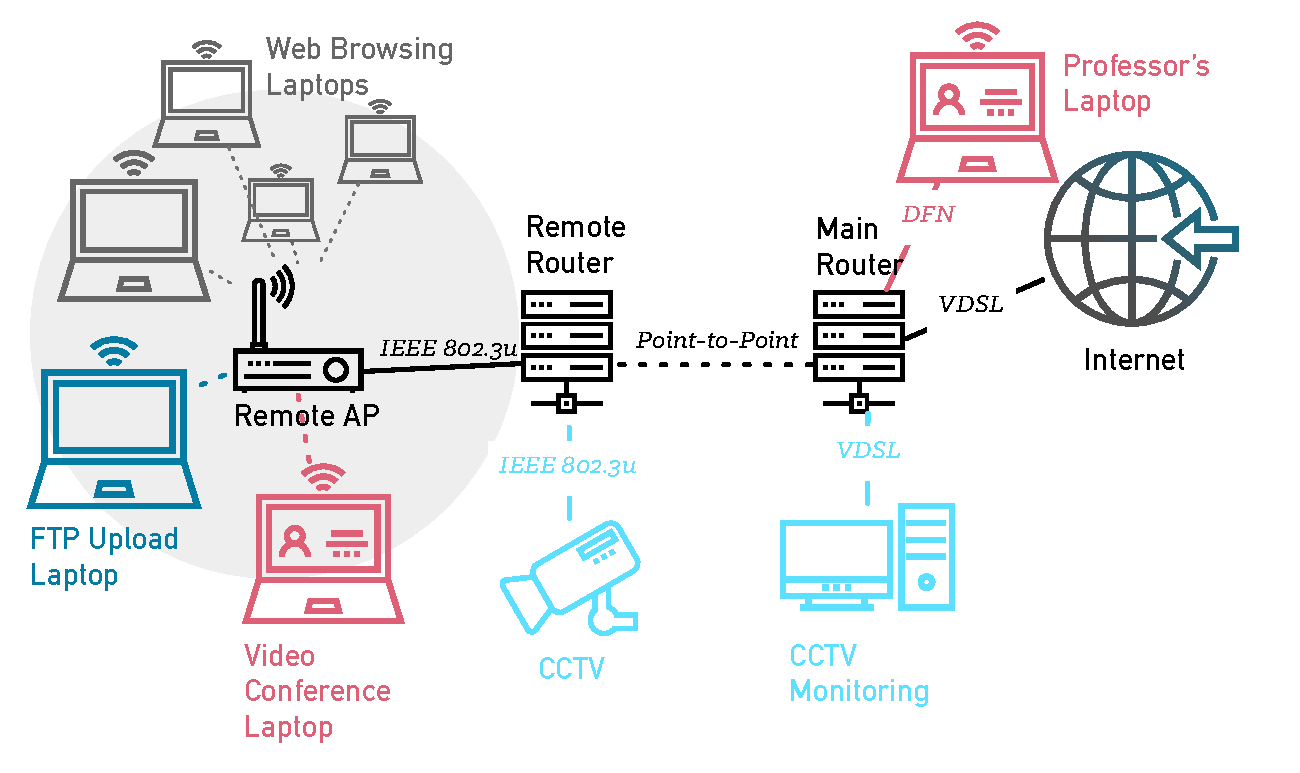
\includegraphics[width=\textwidth]{Figures/network.pdf}
  \caption[asdf]{The Network Setup as simulated.\footnotemark} \label{fig:network}
\end{figure}

\footnotetext{all icons by Icon Fair from the Noun Project.}

To analyze the desired network setup, simulations were conducted. The simulated network was set up as illustrated in fig. \ref{fig:network}. The following section discusses the implementation of the simulation and its configurations.

\subsection{Applications}
\label{subsec:apps}
The network in question contains four different ways of using the network: video conference, FTP upload, web browsing and CCTV. Since all of these traffic types have different characteristics, dedicated applications which model their behavior were created.

\begin{description}
\item[Video conference] The video conference traffic occurring bidirectionally between the Professor's Laptop and the Video Conference Laptop was modeled as a UDP application periodically sending messages of a fixed size. Packets arriving with a delay greater than a fixed maximum delay were discarded and considered lost.
\item[FTP upload] The FTP upload traffic flowing from one student's laptop to the Internet was modeled as a TCP based application which sends as much data at a time as it is allowed by TCP's congestion control algorithms.
The size of the file uploaded using FTP was assumed to be endless, that is: the file upload continued over the course of the entire simulation, no matter the simulation time.
\item[Web browsing] The web browsing traffic generated by all Web Browsing Laptops was modeled as a TCP application which sends HTTP requests of a fixed length to the Internet and receives varying-length responses. The idle period between two requests varies as well.
\item[CCTV] The application modeling the traffic flowing from the CCTV camera to the CCTV monitoring station is based on UDP. Similar to the video conference application, it also periodically sends messages of a fixed size and ignores messages that have been delayed for too long. Its message size is significantly bigger, though, as can be seen in table \ref{table:app_config}.
\end{description}

For a detailed list of specific configuration parameters, see section \ref{sec:conf_details}.

\subsection{Configuration Details}
\label{sec:conf_details}

\begin{table}[H]
\begin{tabularx}{\textwidth}{ l l }
\multicolumn{2}{ l }{\textbf{Video conference application}} \\
\hline
  Message length       & 1388 B payload + 12 B minimal RTP header \\
                       &  = 1400 B\\
  Packet send interval & 40 ms \\
  Maximum packet delay & 100 ms \\
\multicolumn{2}{ l }{\textbf{Web browsing application}} \\
\hline
  HTTP request length  & 8 KiB \\
  HTTP response length & exponential($\mu = 671539$) [see section \ref{subsec:traffic_mod}] \\
  Idle interval        & exponential(20 s) \\
\multicolumn{2}{ l }{\textbf{CCTV application}} \\
\hline
  Message length       & 10KiB \\
  Packet send interval & 40 ms \\
  Maximum packet delay & 100 ms \\
\end{tabularx}
\caption{Application configuration parameters}
\label{table:app_config}
\end{table}

\begin{table}[H]
\begin{tabularx}{\textwidth}{ l l }
\multicolumn{2}{ l }{\textbf{Network}} \\
\hline
  PPP queue size                & 50 frames\\
  WLAN version \& bandwidth     & IEEE 802.11g, 54 Mbit/s \\
  Ethernet version \& bandwidth & IEEE 802.3u, 100 Mbit/s \\
  VDSL bandwidth                & 100 Mbit/s \\
  VDSL delay                    & Internet: 30 ms \\
                                & CCTV Monitoring: 0 ms \\
  DFN bandwidth \& delay        & 100 Mbit/s, 5 ms \\
  Maximum packet loss rate      & 5 \% \\
  (video conference \& CCTV)    & \\
\end{tabularx}
\caption{Network configuration parameters}
\label{table:app_config}
\end{table}

\begin{table}[H]
\begin{tabularx}{\textwidth}{ l l }
\multicolumn{2}{ l }{\textbf{Simulation}} \\
\hline
  Duration          & 1000 s \\
  Repetitions       & 15 \\
  Number of laptops & 1, 5, 10, 15, 20, 30, 40, 50 or 60
\end{tabularx}
\caption{Simulation configuration parameters}
\label{table:app_config}
\end{table}

\subsection{HTTP Traffic modeling}
\label{subsec:traffic_mod}
%TODO: Chi square stuff

To model the size of the HTTP responses, the given trace file was analyzed in order to find a probability distribution that represents their data well.

\begin{figure}[!ht]
  \centering
  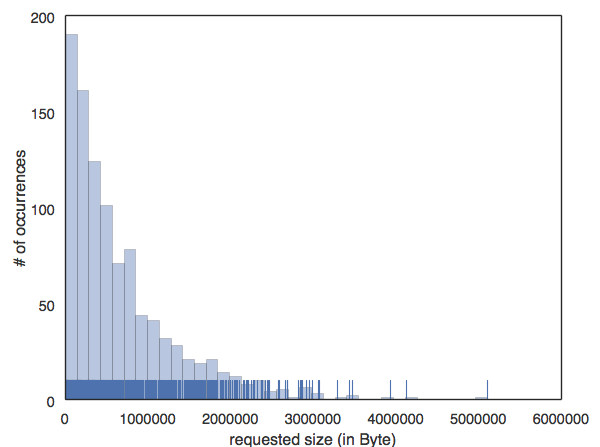
\includegraphics[width=0.7\textwidth]{Figures/trace_plot.png}
  \caption{Frequency of packet sizes found in the trace file} \label{fig:first_plot}
\end{figure}

After plotting the frequency of packet sizes found in the trace file (see Fig. \ref{fig:first_plot}), it was assumed that either a Poisson- or an exponential distribution could be a suitable theoretical distribution. The overall mean of the trace data is 671539.
Using Pearson's $\chi^2$ goodness of fit test, it was determined that, when using an exponential distribution with mean 671539, the null hypothesis can be rejected with a 95\% confidence level:\\

% TODO: zahlen (interval number, interval size) genauer begründen?
First, the sample data was divided into 100 intervals, where intervals with $\leq 5$ values were merged with their neighboring interval until the resulting interval contained more than 5 values, resulting in $k = 45$ intervals of observed data at the end.\\

Then, Pearson's $\chi^2$ test for goodness of fit $\chi^2 = \sum \frac{(Observed - Expected)^2}{Expected}$ was performed for both the Poisson and exponential distribution\footnote{This was done using the Matlab script \texttt{ChiSquareTrace.m} which can be found among the files submitted with this report}. In both cases, $\lambda = 671539$ was used as the function's input value.\\

\textbf{For the exponential distribution,} the resulting values were
\begin{align*}
\chi^2 &= 61.1437\\
\text{p-value} &= 0.0222
\end{align*}
leading to a rejection of the null hypothesis as $p < \alpha = 0.05$.\\
\textbf{For the Poisson distribution,} $\chi^2 = 9.3751 \cdot e^{20}$, suggesting that it is not a good fit.\\

This suggests that the exponential distribution is suitable to generate HTTP response sizes during the simulation.

%TODO: say why poisson doesn't fit?

\subsection{Network behavior}
In the following, the network behavior in terms of traffic and bandwidth utilization will be approximated roughly.
This helps set up the simulation network as described in section \ref{sec:sim_plan} and enables the estimation of the maximum number of Web Browsing Laptops (also needed for the simulation).

\subsubsection{CCTV bit rate}
When sending packets of 10 kB of CCTV data every 40 ms, a bit rate of 2 megabits per second is generated:

\begin{align*}
\text{number of packets per second} &\cdot \text{packet size} = \text{bit rate}\\
\frac{1000ms}{40ms} &\cdot 10kB \cdot 8 bit = 2Mbps
\end{align*}

\subsubsection{Video conference bit rate}
The professor's bidirectional RTP over UDP video conference generates a bit rate of 0,56 megabits per second. In each direction, a bit rate of 0,28 Mbps is achieved:

\begin{align*}
\text{number of packets per second} &\cdot \text{packet size} = \text{bit rate}\\
\frac{1000ms}{40ms} &\cdot 1400B \cdot 8 bit = 0,28 Mbps
\end{align*}

Where the 1400B packet size are 1388 B payload + 12 B minimal RTP header.\\

In conclusion, a total $2\text{Mbps} + 2 \cdot 0,56 \text{Mbps} = 2,56 \text{Mbps}$ of the point-to-point radio link's bandwidth are used constantly.

\subsubsection{FTP upload bit rate}
Since the FTP file transfer is a bulk upload rather than a continuous data stream, its bandwidth usage is not constant. Using TCP's congestion avoidance algorithms, the TCP connection taking care of the transfer will attempt to use as much of the available bandwidth as possible (until collisions occur). Therefore, the FTP traffic is not part of the network's baseline traffic.

%----------------------------------------------------------------------------------------
%	METHODS
%----------------------------------------------------------------------------------------

\section{Simulation Plan}
\label{sec:sim_plan}

The overall goal of the simulation is to evaluate how the previously described applications perform and what the bottlenecks of the network are. First we identified potentially changing parameters of the network. These are the variables we can modify between different simulation runs. Afterwards we identified critical performance characteristics of the applications and performance metrics of the potential bottlenecks.

\subsection{Simulation Parameters}
The first parameter to look at is the amount of web browsing clients. We expect a decreasing performance with the amount of clients rising.
The second part is the CCTV. To determine the influence of the CCTV on the network performance, we either include or exclude the CCTV from the simulation.

To determine the maximum number of clients to simulate, we looked at the scenario itself. An amount of 60 clients is a reasonable amount of students to be present in a $400m^{2}$ area. It can be assumed that they are surfing at the same time, if the lecture requires web research. To analyze the network thoroughly though, we need to make sure that the behavior with more clients does not change significantly. We found that it is not expected, that the behavior of the system changes significantly at a higher amount of clients, so we are able to extrapolate several network properties from the simulation results.
To be able to extrapolate properly, we need to determine the incrementation of the amount of clients as well. To receive a well formed graph, we should work with a low increment, when the network behavior changes significantly. At low numbers, the traffic share is higher, therefore we need a low increment. At higher numbers we can increase it. The resulting numbers of clients we simulated are:
\begin{align*}
N \in \{1,5,10,15,20,30,40,50,60\}
\end{align*}
To find a suitable duration of the simulation, we need to examine the behavior over time. We identified the browsing clients as the only application, whose behavior is depending on time. The mean time between HTTP requests is 20 seconds and it is exponentially distributed. The mean reply length is 671539 bytes and it is exponentially distributed as well. To get good results, we should include a high range of possible values in the simulation time. To calculate a reasonable expected highest value to take into account, we used the cumulative distribution function(CDF) of the exponential distribution:
\begin{align*}
y = 1-e^{-{\frac{1}{\mu}x}}
\end{align*}
If we want to include 95\% of the random values, we need to calculate the upper bound of the waiting time and the reply length, by applying the CDF:
\begin{align*}
{-ln(0.05)} * 671539 B \approx 2MB
\end{align*}
\begin{align*}
{-ln(0.05)} * 20s \approx 60s
\end{align*}
Our simulation showed, that the throughput for 60 clients goes down to 80000 bps. The expected time from simulation start to the end of the first request is therefore:
\begin{align*}
\frac{8\frac{b}{B} * 2MB}{80000 bps} + 60s = 260s
\end{align*}
To allow more of these requests, we set the maximum simulation time to 1000 seconds.

Throughout the simulation, we looked at the confidence intervals of several averaged values. We found that a repetition of 15 for each simulation combination produces sufficiently small intervals at a confidence level of 95\%.

For the final simulation we end up with 9 different client and 2 CCTV settings, resulting in 270 simulation runs with a simulation duration of 1000 seconds.

\subsection{Performance Characteristics} \label{performance_characteristics}
In the previous section we determined changing parameters between the simulation runs. The performance characteristics are the simulation measurements influenced by those parameters. The overall procedure is to record the measurements for every combination of parameters several times. Thus we have a set of 15 measurements for each combination. This allows us to calculate confidence intervals for each measurement. In the following we identify the performance characteristics of the implemented applications.

\subsubsection{Video Conference}
The video conference is based on UDP. Therefore packets can be dropped by the network permanently, reducing the quality of service. Additionally packets can be delayed. If a packet arrives too late, it can't contribute to the video stream anymore and is thus considered lost. The limit for the packet delay is 100 ms. If the packet loss rate is higher than 5\%, the quality of the video conference is considered to be too bad. Thus the crucial characteristic to look at is the average packet loss rate of the video conference in both directions.
Another characteristic is the average delay. Although you could expect it to be below 100 ms, when the average packet loss rate is sufficient, it is still an important value to rate the quality of service.
\begin{align*}
\frac{\text{lost packets} + \text{discarded packets}}{\text{sent packets}}
\end{align*}
\subsubsection{Web Browsing}
The web browsing follows a simple request response model. The requests are carried out in a single session each. The important characteristic is how long the user has to wait until a response arrives. The response time is depending on the length of the response. For a greater length the user can cope with a longer response time. Therefore the crucial characteristic is the throughput the web client actually achieves.
It is possible to measure the average throughput of the web clients. But this value is misleading, since the browsers do not use the medium at all times. To address this issue we measured the fraction of the simulation time a session was active. The calculation of the final throughput is thus:
\begin{align*}
\frac{1}{N}\sum_{i=1}^{N}\frac{r_{i}}{f_{i} * T}, \\
\text{where}~N &= \text{number of clients,} \\
r &= \text{received bits,} \\
f &= \text{fraction of the overall time,} \\
T &= \text{overall simulation time}
\end{align*}
To estimate the average response time, we can then further divide the average response length by the just acquired value.
Todays response times for common home networks are usually below 5 seconds. For a temporary back-up solution such as the network at hand slightly higher response times can be considered acceptable. Therefore you can say that it is okay to wait for a response for 10 seconds.

\subsubsection{FTP Upload}
The FTP Upload is modeled as a continuous TCP stream to the Internet. It runs for the entire simulation. The only important characteristic is the average throughput. The user is just interested in the time the upload takes. We measured the average throughput by the total amount of bytes uploaded to the server divided by the simulation time.
\begin{align*}
\frac{\text{uploadedBits}}{\text{simTime}}
\end{align*}

\subsubsection{CCTV}
The CCTV is used to monitor abnormal behavior at the remote campus. There are two characteristics, which can be considered. At first the delay of stream increases the reaction time of the staff. If the information arrives at the monitor one second late, it does not influence the reaction time of the staff in a significant way. Therefore it is negligible.
As of the conference the average packet loss rate influences the quality of the video stream. If the packet loss rate is higher than 5\% the video stream is considered not to be recognizable anymore. Therefore the packet loss rate should not exceed 5\%.

\subsection{Bottleneck Identification}
Besides looking at the performance characteristics of the application, it is advisable to look at potential bottlenecks. We identified the wireless network at the remote campus and the radio link between the remote campus and the main campus as potential bottlenecks. The theoretical maximum bandwidth of 56 Mbps of the wireless network and a 12 Mbps bandwidth of the radio link are much smaller than the bandwidths of the remaining links. Thus it is not necessary to evaluate those.

\subsubsection{Radio Link}
To evaluate the radio link we need to consider two different characteristics. It is useful to determine how much bandwidth of the link is unused. Therefore we need to measure the average throughput. To receive even more information, we can look at the throughputs in each direction of the link. So we can identify the potential application, which is causing the traffic.
In case the link is indeed a bottleneck, it is necessary to collect data about the packet drop rate. When the link is overloaded, the packets will be hold in a queue. When this queue is full. Incoming packets are dropped. We can use this drop rate to determine, if the link is a bottleneck.
Since our applications require a sufficient packet delay, it is also useful to record the average queueing delay, to evaluate the influence of the link on the streaming delays.
All of these measurements can be done at the Remote Router and Main Router to distinct between traffic directions.

\subsubsection{Wireless Network}
The practical throughput of a wireless network is much lower than the advertised theoretical maximum. This is due to collisions on the channel. So the wireless network can still be considered as a potential bottleneck, while its theoretical maximum bandwidth 56 Mbps is much higher than the 12Mbps of the radio link. To evaluate the wireless network channel, the same statistics as of the radio link can be considered.
Additionally it is useful to look at the number of collisions to have a good metric to assess the issues caused by the channel.

\section{Simulation Evaluation}
The following sections contain the separated evaluation of the network with and without CCTV.
We would like to mention that we did the simulation with an important change of a parameter increasing primarily the performance of all applications depending on short network delays. We reduced the maximum PPP queue length to 50. We found, that large packets of the CCTV cause a tremendous amount of queueing delay due to high transmission delays of queued up packets. By decreasing the queue size the impact of accumulated CCTV packets at the Remote Router queue on the video conference is decreased.

\subsection{Network with CCTV}
This section contains the final evaluation of the network, when CCTV is included. We will start with an overview of the network behavior to be able to explain the behavior of the applications. After evaluating the application performances we continue with identifying and explaining bottlenecks.
\begin{figure}[!ht]
  \centering
  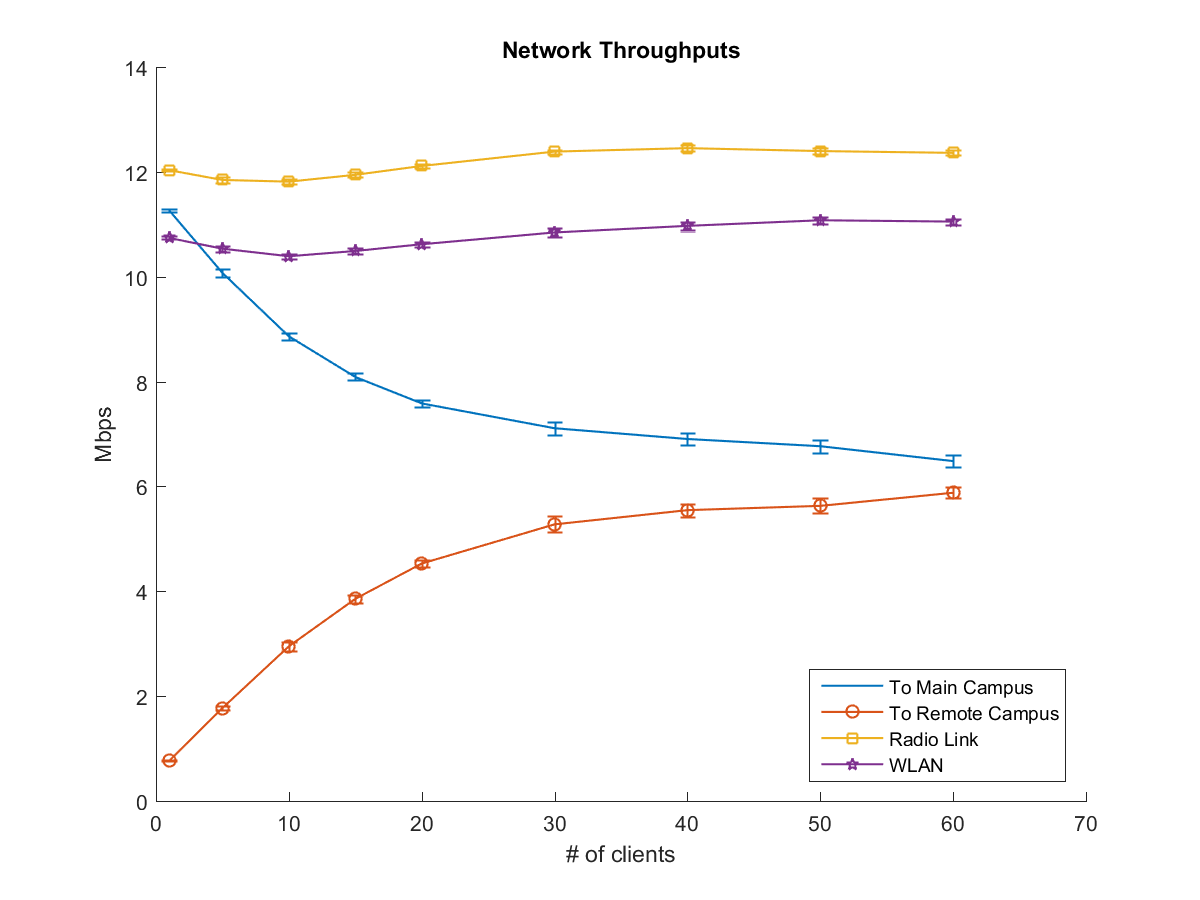
\includegraphics[width=\textwidth]{Figures/cctv/Network_Throughputs.png}
  \caption{Throughputs of the important links of the simulated network including confidence intervals at a confidence level of 95\%.} \label{fig:cctv_network_throughputs}
\end{figure}

The network throughputs are depicted in fig. \ref{fig:cctv_network_throughputs}. As expected the total rate of the radio link is slightly above the rate of the WLAN. This is due to the steady load, which is added directly by the CCTV stream. The remaining bandwidth is composed of the steady load of the video conference, the web browsing and FTP upload traffic. With a rising number of clients the traffic directed to the main campus decreases and the traffic to the remote campus increases. This can be explained by looking at the application throughputs depicted in \ref{fig:cctv_app_throughput_all}. With more clients the HTTP traffic uses a higher share of bandwidth. In general one can argue, that the major amount of HTTP traffic flows in the direction of the remote campus, while the traffic of the FTP upload flows to the main campus.
\begin{figure}[!ht]
  \centering
  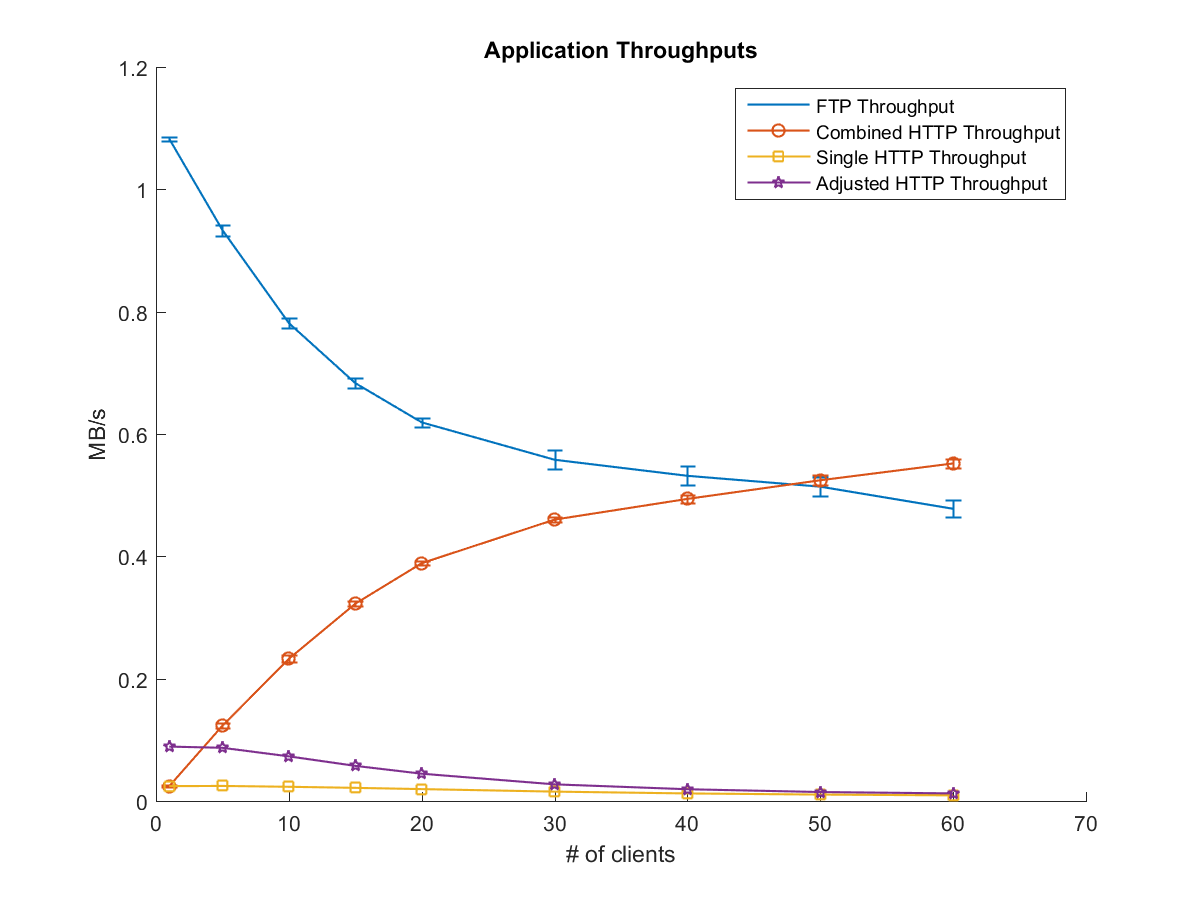
\includegraphics[width=\textwidth]{Figures/cctv/Application_Throughputs.png}
  \caption{Average throughputs of the applications of the simulated network including confidence intervals at a confidence level of 95\%.} \label{fig:cctv_app_throughput_all}
\end{figure}
\subsubsection{Application Performance}
In section \ref{performance_characteristics} we identified the important performance characteristics of the implemented applications. In this section we will step through them and apply the simulation results.

The performance of the browsers and FTP upload is depending only on the throughput. The application throughputs were previously depicted in fig. \ref{fig:cctv_app_throughput_all}.
The FTP throughput is comparably high at every number of clients. When a low number of clients is surfing, the FTP upload almost uses the whole available bandwidth of the radio link. Only the steady load of the conference and the CCTV is slowing it down. With a bitrate of roughly 9 Mbps to 4 Mbps a good quality of service is achieved. But it is to be expected, that the FTP throughput decreases further with the number of clients rising above 60. Since a higher number of browsing clients does not fit the scenario, the FTP data rate does not set a maximum amount of clients.

The important value of the data rates of the browsing clients is actually the data rate for a single HTTP request. These values are depicted in fig. \ref{fig:cctv_http_request_throughput}.
\begin{figure}[!ht]
  \centering
  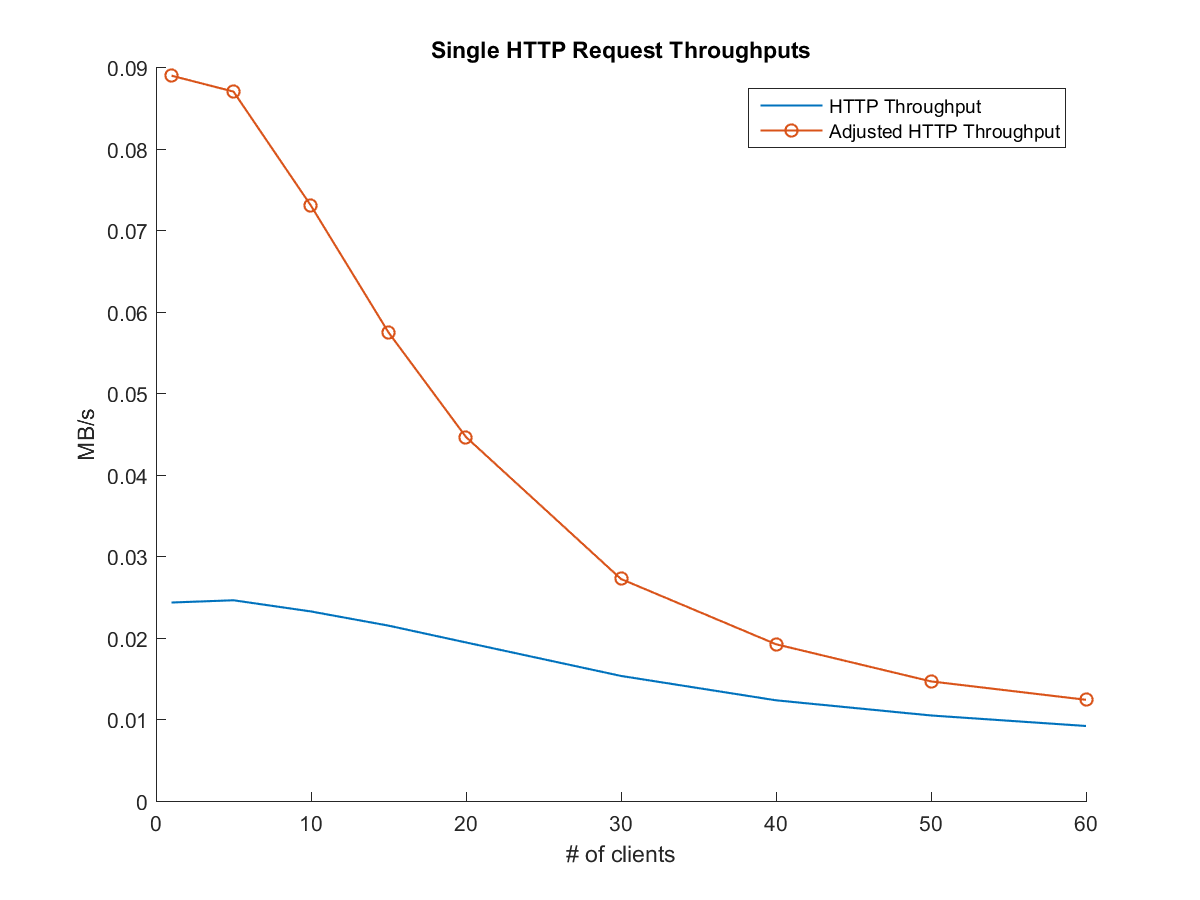
\includegraphics[width=\textwidth]{Figures/cctv/Single_HTTP_Request_Throughputs.png}
  \caption{Throughput of a single HTTP request. The adjusted throughput takes into account the time a request was actually active.} \label{fig:cctv_http_request_throughput}
\end{figure}
\begin{figure}[!ht]
  \centering
  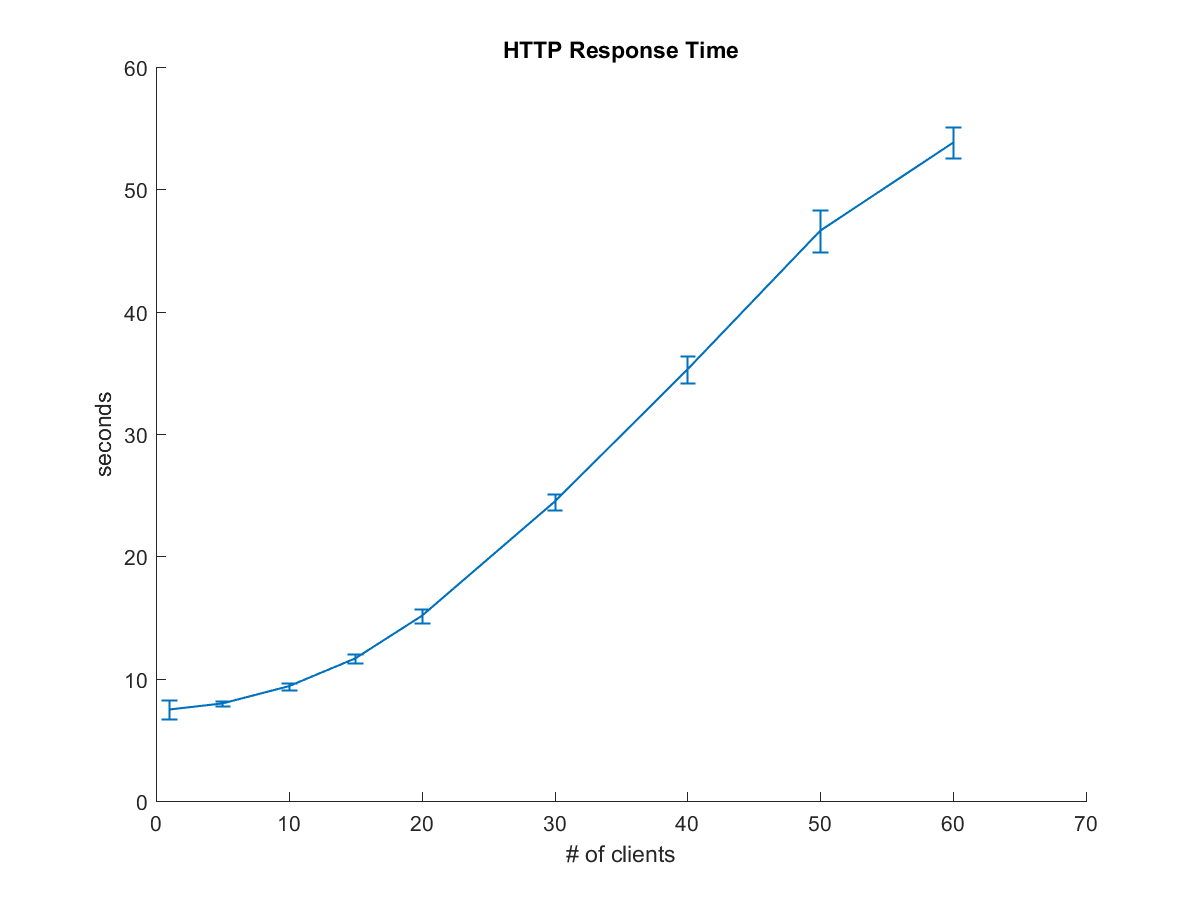
\includegraphics[width=\textwidth]{Figures/cctv/HTTP_Response_Time.png}
  \caption{Response Time of a single HTTP request.} \label{fig:cctv_http_request_time}
\end{figure}

The adjusted data rate is calculated by applying the time a session was actually active instead of the whole simulation time.

If only one to five clients are using the network a comparably high data rate of roughly 100 KB/s is achieved. In combination with a mean reply length of 672 KB this results in an average waiting time of 6.7 seconds. This is already a really bad experience. You can argue that it is acceptable at the given circumstances. We argued before that an average waiting time of 10 seconds is acceptable in these circumstances. This time is exceeded, when more than 10 clients are using the network. The average HTTP Response Time is depicted in fig. \ref{fig:cctv_http_request_time}. Therefore 10 clients provide a maximum of the proposed network configuration.

The performance characteristics of the video conference and the CCTV are the packet loss ratio and packet delays. The simulation results are depicted in fig \ref{fig:cctv_app_packet_loss_rates} and \ref{fig:cctv_app_packet_delays} respectively.
\begin{figure}[!ht]
  \centering
  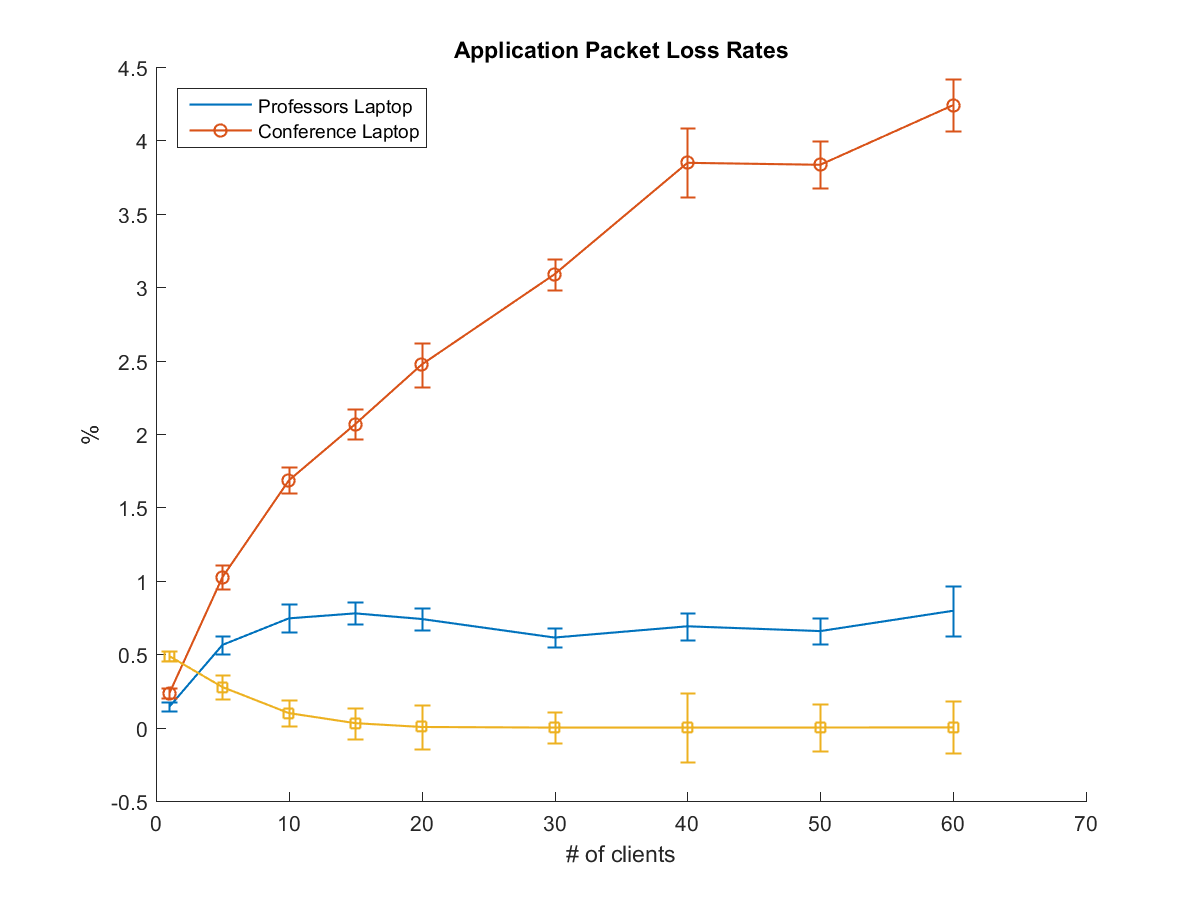
\includegraphics[width=\textwidth]{Figures/cctv/Application_Packet_Loss_Rates.png}
  \caption{Packet loss rates of the applications of the simulated network including confidence intervals.} \label{fig:cctv_app_packet_loss_rates}
\end{figure}

The packet loss rates of the CCTV stream starts at a comparably high packet loss rate and decreases up to 0 for a higher number of clients. When a low number of clients is using the network almost all TCP traffic is directed to the main campus. Therefore the congestion at the radio link causes the queues at the Remote Router to drop packets. Therefore increasing the packet loss rate of the CCTV stream. A packet loss rate of 5\% is not exceeded at any amount of clients. Therefore a good quality is to be expected.

The packet loss rate of the stream directed to the professors laptop is low for a small number of clients and increases up to a rate of roughly 0.7\% at 10 clients and keeps steady from there on. A possible explanation for the low loss rate at the beginning, while the loss rate for CCTV is high is, that the packet size of the video stream is much smaller than the CCTV stream packet size. While the CCTV packets arrive late due to transmission delay the video stream packets arrive faster and are therefore not considered lost.

The before mentioned loss rates are far below our threshold of 5\%. Therefore they are not a limiting factor on the network. The packet loss rate of the stream received by the conference laptop however reaches a value of 4.2\% at 60 clients. The overall graph suggests, that the 5\% mark is exceeded at about 90 clients. Since 90 clients are an unrealistic number of clients considering the scenario, the performance of the stream can still be considered acceptable. The increase of the packet loss rate is caused by the increasing amount of traffic directed to the remote campus clients and therefore causing packet drops at the Main Router and access point queues.
\begin{figure}[!ht]
  \centering
  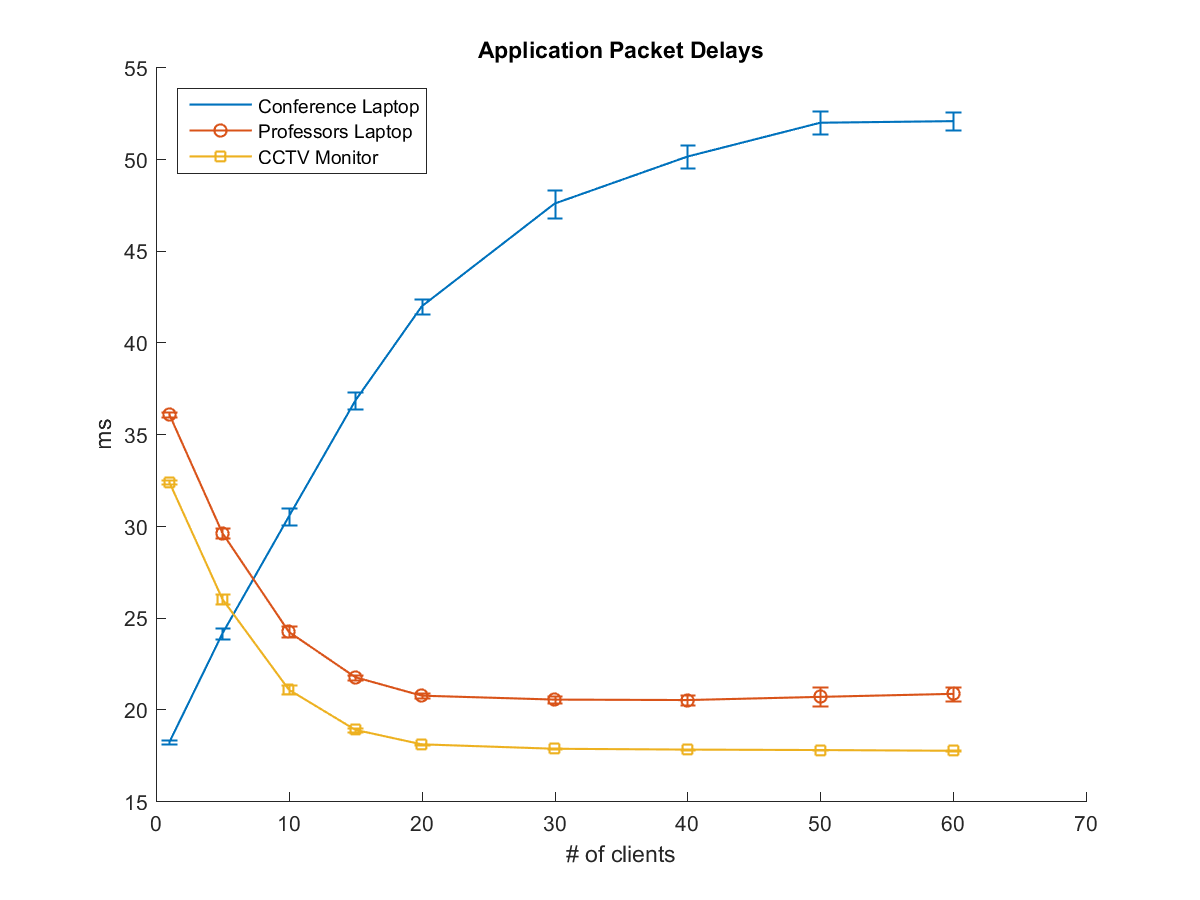
\includegraphics[width=\textwidth]{Figures/cctv/Application_Packet_Delays.png}
  \caption{Average packet delays of the applications of the simulated network including confidence intervals.} \label{fig:cctv_app_packet_delays}
\end{figure}

The delay depicted in figure \ref{fig:cctv_app_packet_delays} is constantly low enough to be considered acceptable. The inverse behavior of the delays is caused by the direction of the expected traffic. At low client numbers only the queue at the Remote Router delays the packets. With an increasing number of clients the access point and the Main Router delay the packets due to the HTTP replies.

\subsubsection{Bottleneck Analysis}
The overall throughput of the network components was previously depicted in fig. \ref{fig:cctv_network_throughputs}. It shows that the radio link bandwidth is fully used at every number of clients. This is due to the TCP traffic caused by the FTP upload. The TCP protocol is designed to use all remaining bandwidth not used by steady load of the udp traffic. Since all TCP traffic is originated at the WLAN part of the network, it is expect that the WLAN throughput equals the throughput of the radio link without the steady load of the CCTV, which is connected directly to the Remote Router.
The packet drop rates of the network queues are depicted in fig. \ref{fig:cctv_netw_packet_drop_rates}.
\begin{figure}[!ht]
  \centering
  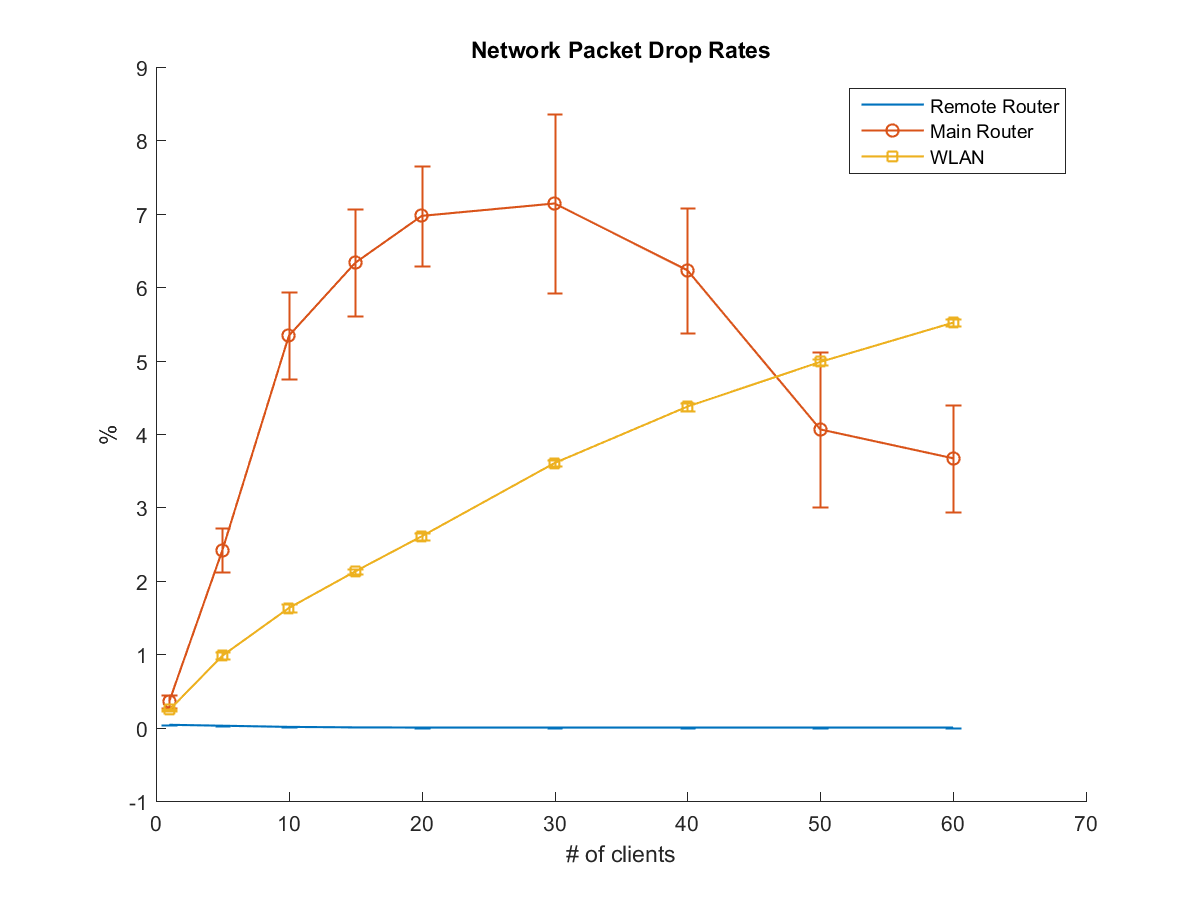
\includegraphics[width=\textwidth]{Figures/cctv/Network_Packet_Drop_Rates.png}
  \caption{Average packet drop rates of the simulated network including confidence intervals.} \label{fig:cctv_netw_packet_drop_rates}
\end{figure}

The drop rate of the WLAN is increasing monotonously, while the Main Router drop rate increases more steeply, but decreases at a higher number of clients. The Remote Router queue is around zero regardless. This is due to the fact, that the main TCP traffic directed to the main campus is the FTP upload. Since it is only one stream, it can perfectly adapt to the available bandwidth. Furthermore it indicates that the WLAN is used at maximum capacity, because even the 8KiB HTTP requests should cause congestion at the Remote Router. The WLAN is therefore filtering the traffic originating from the remote campus. So the packets actually reaching the Remote Router do not get dropped anymore. This means a usable capacity of the WLAN of 10Mbit, which is the bandwidth of the radio link minus the data rate of the CCTV.

The steep increase of the drop rate at the main router indicates the impact of the HTTP requests. When a request reaches the internet, the server initiates a reply, which causes a congestion at the main router, because the radio link is fully in use at all times. With a low number of clients the increase of requests is primarily linear. Therefore the drop rates at the main router increase linearly as aswell. With the number of clients however the share of the bandwidth of each client decreases, this results in a longer session duration. A longer session duration means a decrease of the number of requests, since no new request is issued before the current request got served. This opposed effects increase the congestion at the main router up to 10 clients linearly. Afterwards the secondary effect decreases the congestion caused by the primary effect, resulting in a logarithmic behavior of several curves. For instance the packet drop rate at the WLAN access point. The queues at the access point and the main router contain the same traffic. Since the congestion at the access point continously rises, the access point reduces the request throughput, which causes the congestion and therefore drop rate of the main router to finally go down, when 30 web clients and more use the network.
With more than 30 to 40 clients, the access point and therefore the WLAN takes over the role of the crucial bottleneck.
Since the UDP traffic directed to the conference laptop and the vast amount of traffic generated by the HTTP requests traverse the exact same queues, the resulting throughputs and packet drop rates are closely related.

\begin{figure}[!ht]
  \centering
  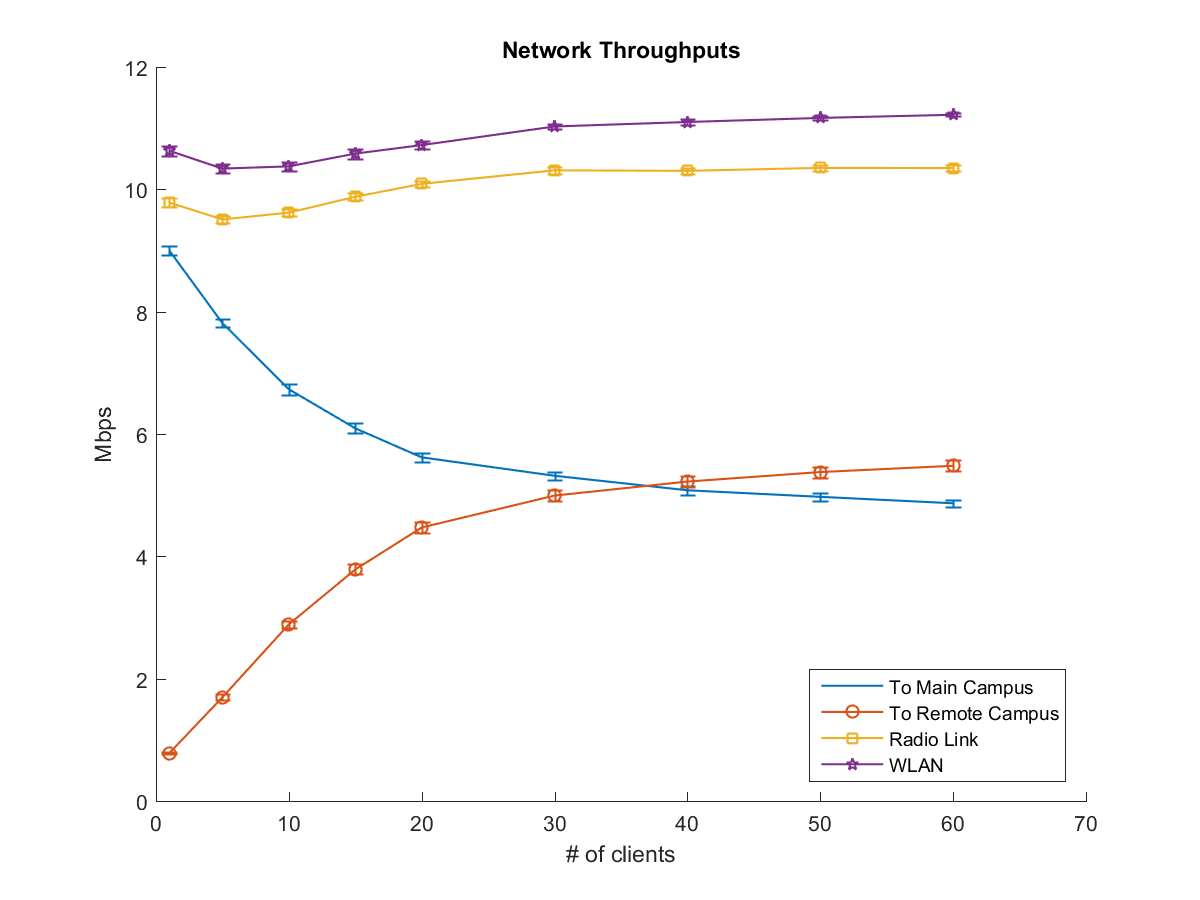
\includegraphics[width=\textwidth]{Figures/nocctv/Network_Throughputs.png}
  \caption{Average network throughputs} \label{fig:net_throughput}
\end{figure}

\subsection{Network without CCTV}
As a second measure, the same simulations were conducted without any CCTV infrastructure present. This section analyzes the simulation results of this configuration. First, the overall network behavior is discussed. Then, it focuses on the influence of FTP and web browsing applications on the video conference. Finally, possible bottlenecks are identified. Note that all confidence intervals displayed in the following have a confidence level of 95\%, as stated in \ref{sec:sim_plan}.

\subsubsection{Overall network behavior}

The throughput at different points in the network is illustrated in fig. \ref{fig:net_throughput}. It can be observed that the radio link is never at full capacity. The traffic towards the Main Campus represents the sum of the FTP upload, HTTP requests and video conference traffic from conference laptop to professor. The traffic towards the Remote campus represents the sum of HTTP responses and video conference data from the Professor's Laptop towards the conference laptop. It can be seen that the throughputs are mostly inverse to each other, forming a steady ceiling of about 10 Mbit/s for $\geq$ 30 clients.\\

\begin{figure*}[!ht]%
\makebox[\linewidth][c]{%
    \centering
    \subfloat[Average queue length\label{fig:rap_queue_len}]{{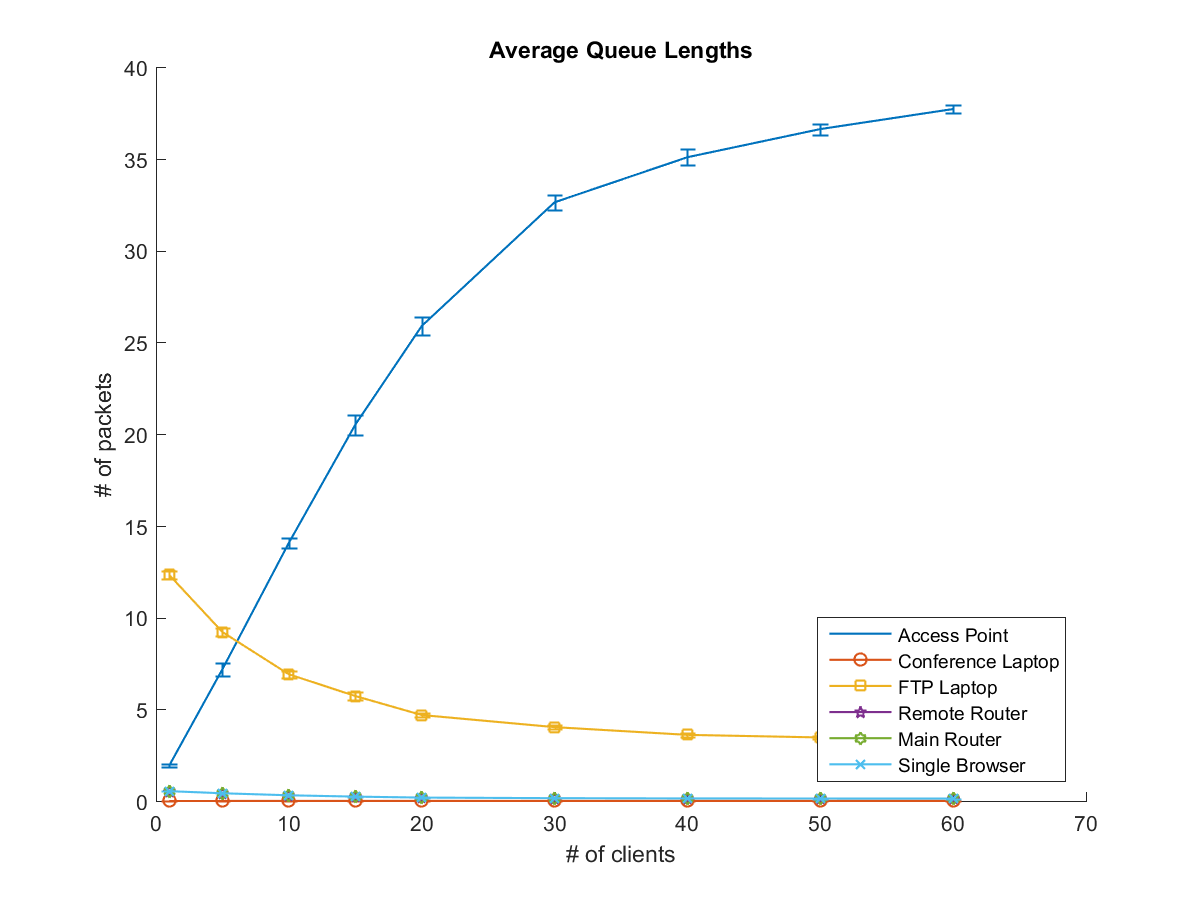
\includegraphics[width=0.85\textwidth]{Figures/nocctv/Average_Queue_Lengths.png} }}\hspace{-2.5em}%
    \subfloat[Number of collisions in the WLAN \label{fig:rap_collisions}]{{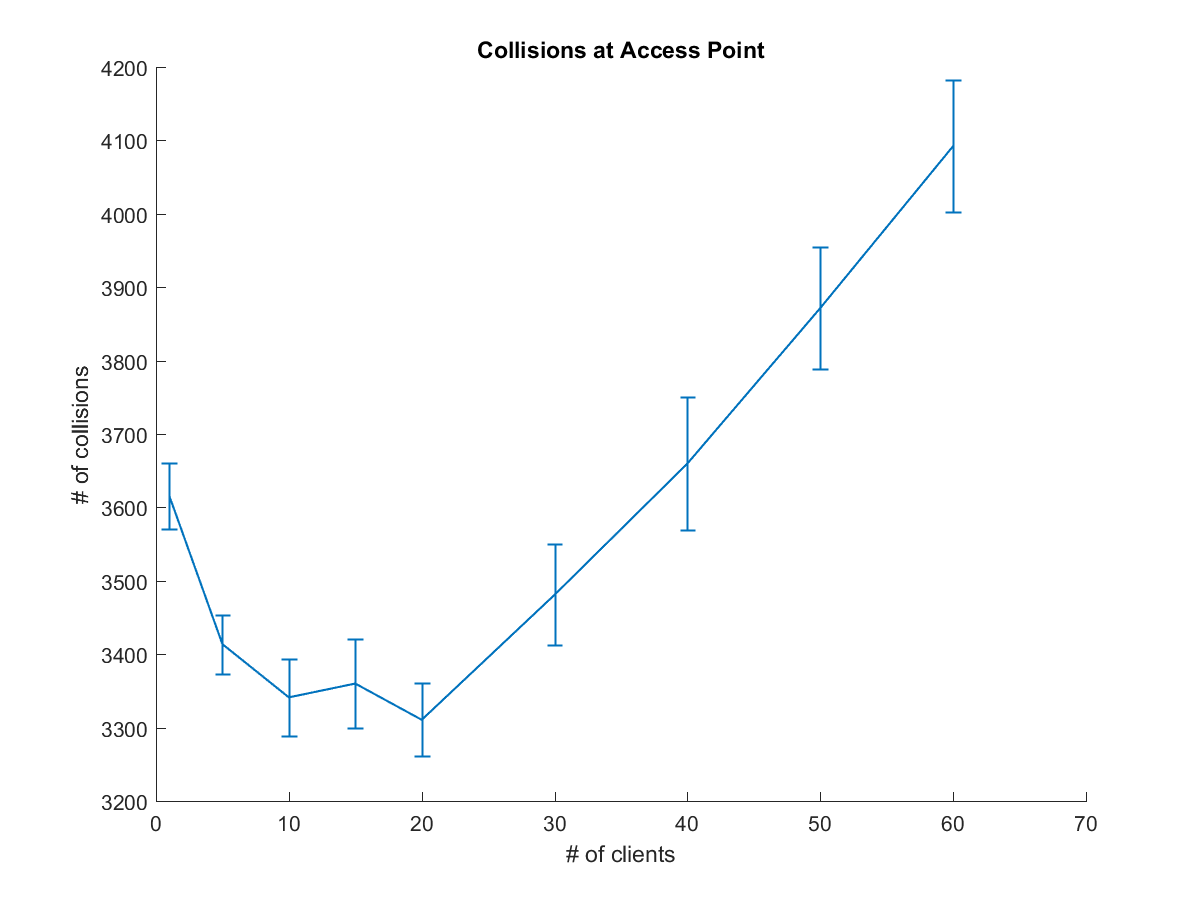
\includegraphics[width=0.85\textwidth]{Figures/nocctv/Collisions_at_Access_Point.png} }}%
  }
    \caption{Remote Access Point data}%
    \label{fig:rap_data}%
\end{figure*}

Due to the aforementioned ceiling, it is worthwhile to inspect the WLAN and the Remote Access Point serving it more closely. As fig. \ref{fig:rap_queue_len} shows, the Remote Access Point queue length, i.e. the amount of data waiting to be sent to the WLAN clients, is the longest quickly after more than 5 HTTP clients have joined the network.

\begin{figure*}[!ht]%
\makebox[\linewidth][c]{%
    \centering
    \subfloat[Average application throughput\label{fig:app_throughput}]{{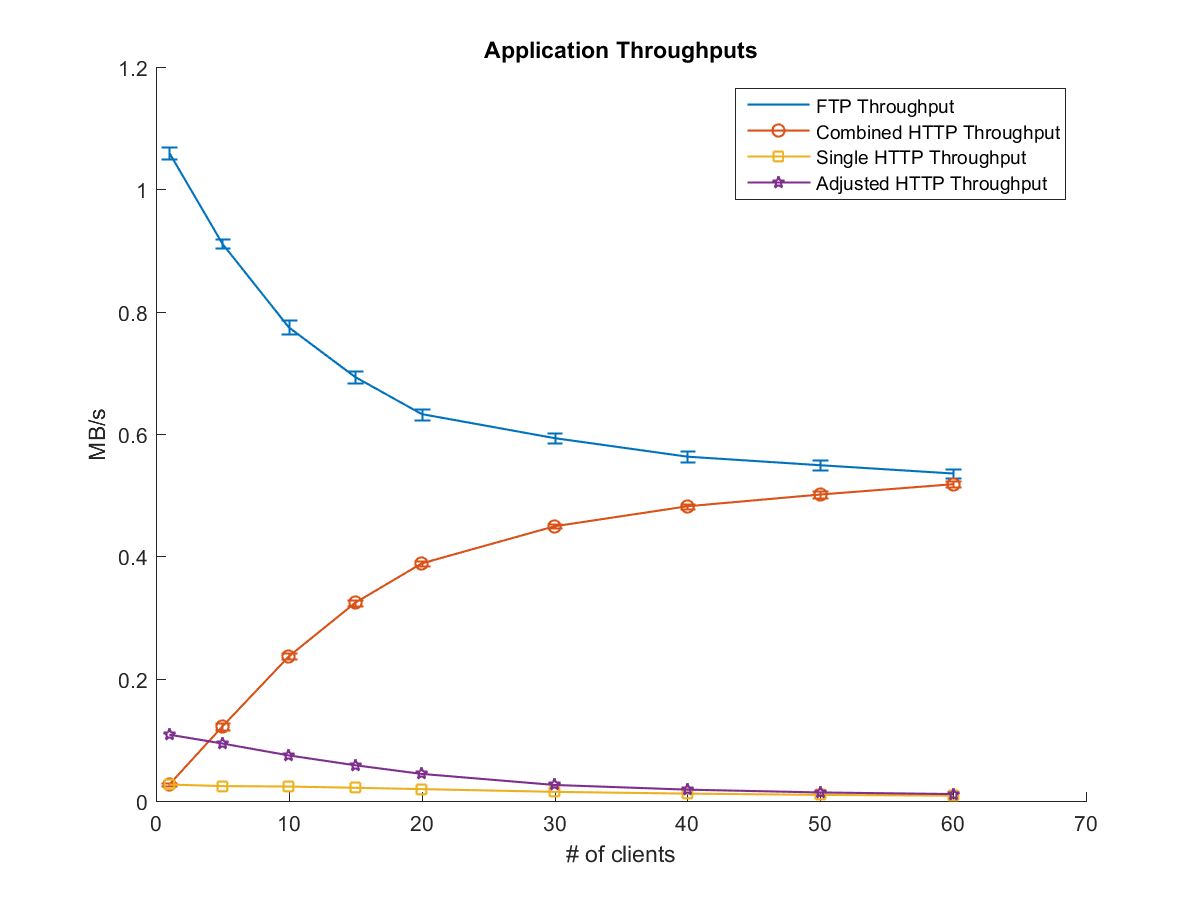
\includegraphics[width=0.85\textwidth]{Figures/nocctv/Application_Throughputs.png} }}\hspace{-2.5em}%
    \subfloat[Average browser session durations \label{fig:browser_sess_dur}]{{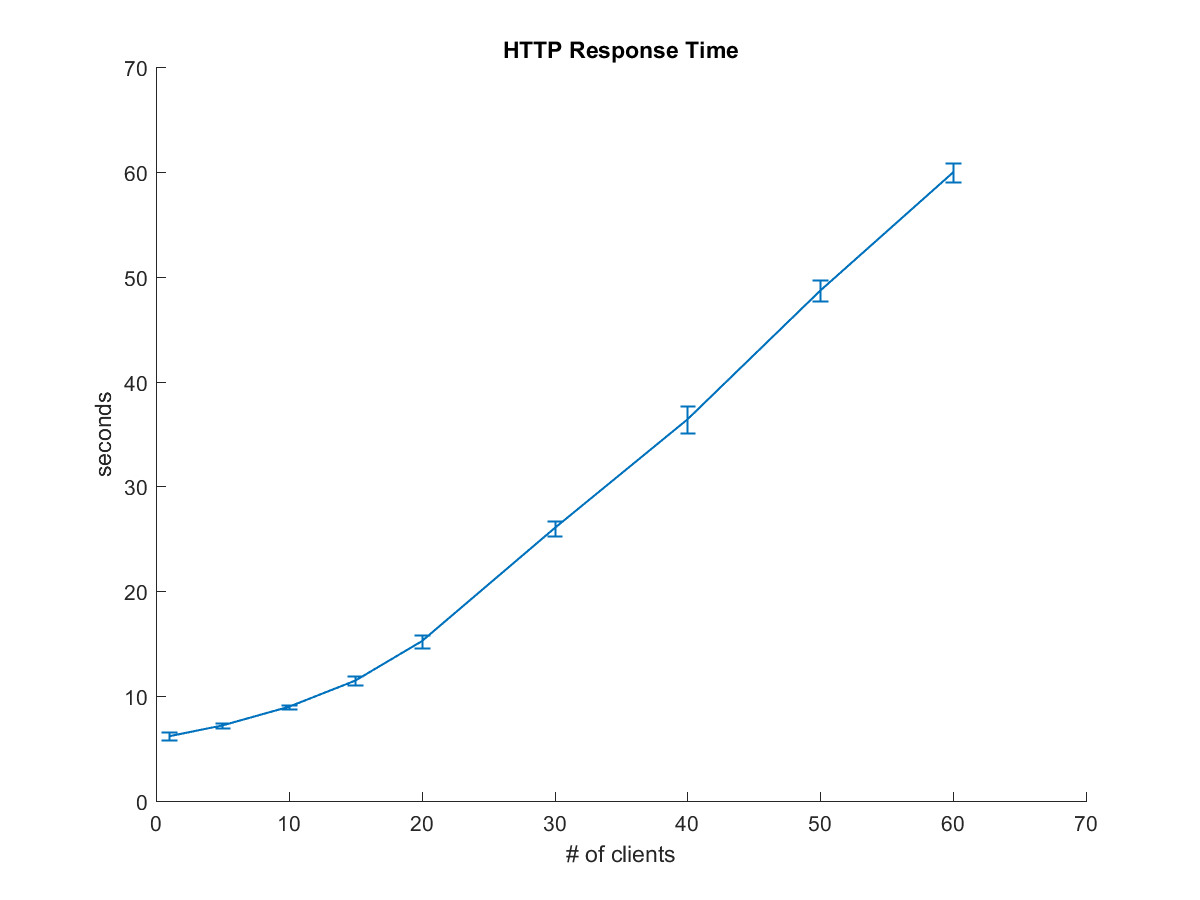
\includegraphics[width=0.85\textwidth]{Figures/nocctv/HTTP_Response_Time.png} }}%
  }
    \caption{Application data}%
    \label{fig:app_data}%
\end{figure*}


Fig. \ref{fig:app_throughput} summarizes the average application throughput with regard to the number of web browsing clients present in the network. In order to analyze the influence of the FTP and web browsing applications on the video quality, it is useful to first familiarize ourselves with the behavior of these applications.

\paragraph{The Web browsers} are the parameter continuously changing throughout the simulation, as detailed in section \ref{sec:sim_plan}. Figure \ref{fig:app_throughput} shows that while the average overall HTTP traffic throughput rises with the number of web browsing clients, the average throughput achieved per browser decreases. Since bandwidth is limited, the TCP congestion control of each participant will negotiate a transmission rate that avoids collisions, throttling the overall transmission speed. Fig. \ref{fig:browser_sess_dur} verifies this: The average session duration per browser increases with the number of clients. According to the criteria determined in \ref{performance_characteristics}, browsing quality declines quickly: At less than 15 active clients, the quality threshold of 10 s is surpassed. Notably, the session duration grows linearly with $\geq$ 20 clients in the network.

\paragraph{The FTP client}, shown in fig. \ref{fig:app_throughput} as well, experiences a %(TODO: characteristic)
decline in throughput that is inverse to the increase in overall HTTP throughput. This also can be explained with TCP's congestion control mechanisms: the more bandwidth is used by web browsing clients, the more the FTP client is forced to react by limiting its bandwidth in order to avoid collisions. In short: the FTP client will use up as much bandwidth as you let them. It can be argued that the decrease in bandwidth is not as much of a nuisance as it is for the web browser users, since large file transfers are expected to take a while anyway.

\begin{figure*}[!ht]%
\makebox[\linewidth][c]{%
    \centering
    \subfloat[Packet loss rates\label{fig:ploss}]{{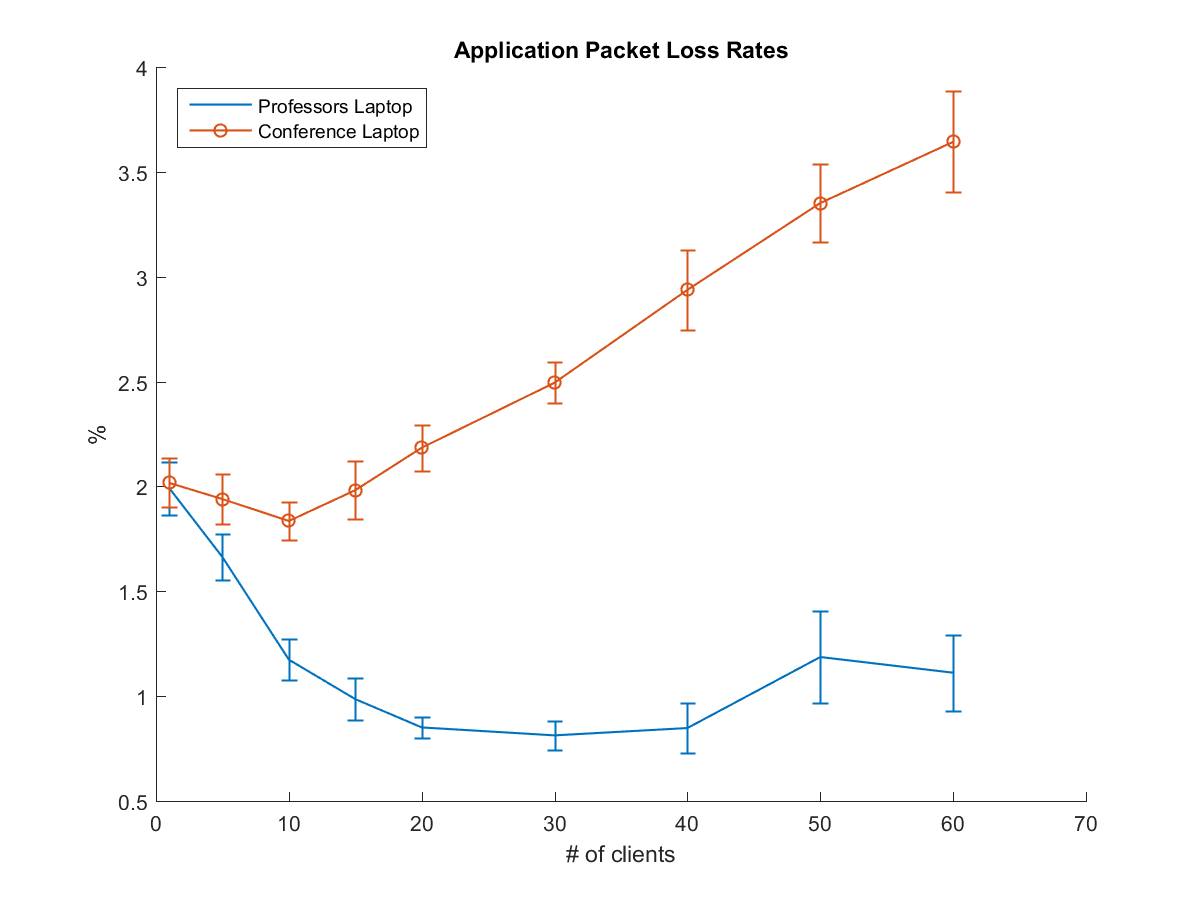
\includegraphics[width=0.85\textwidth]{Figures/nocctv/Application_Packet_Loss_Rates.png} }}\hspace{-2.5em}%
    \subfloat[Delays]{{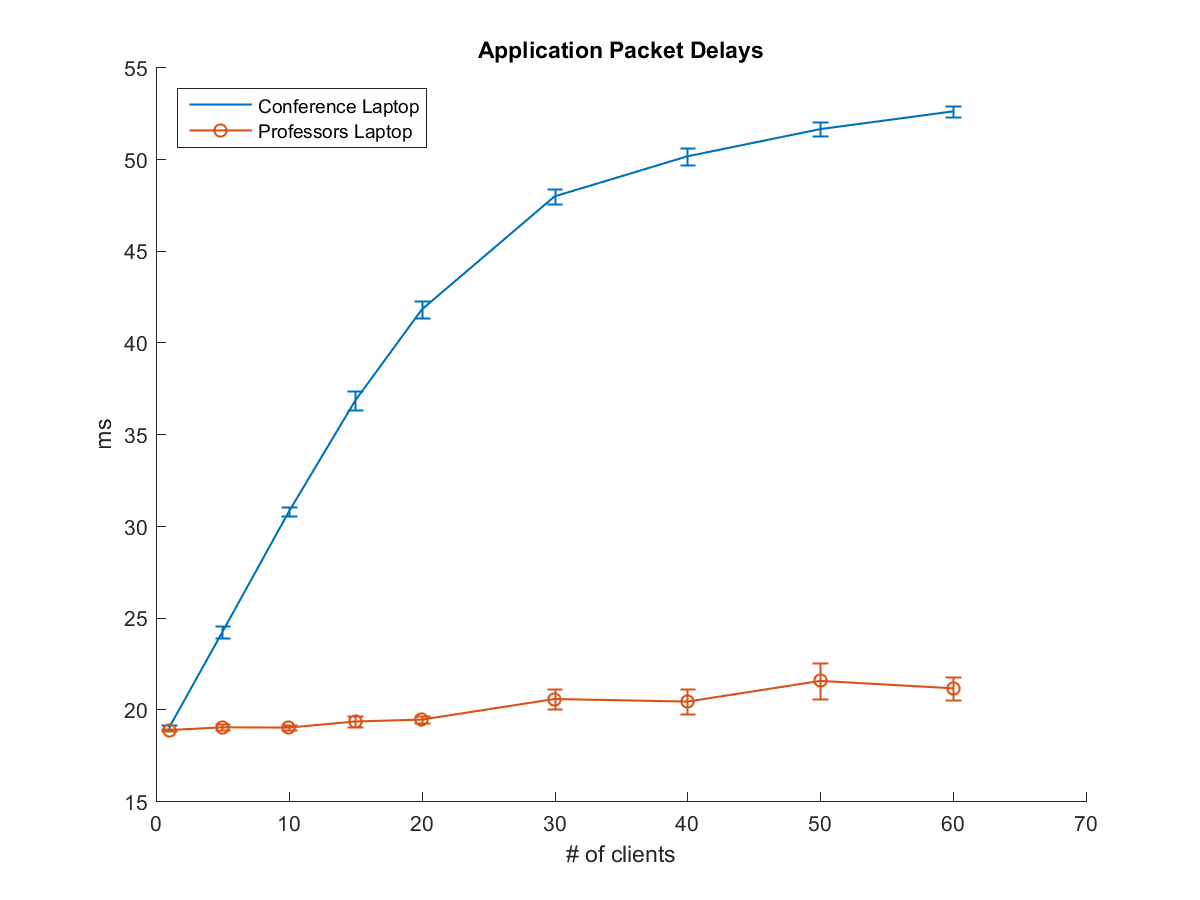
\includegraphics[width=0.85\textwidth]{Figures/nocctv/Application_Packet_Delays.png} }}%
  }
    \caption{Average packet loss and delays of the video conference}%
    \label{fig:conf_data}%
\end{figure*}

\paragraph{The video conference} has to be looked at as two distinct data flows: one going from the Professor's Laptop to the Video Conference Laptop, and one traveling the other way. This becomes apparent when looking at fig. \ref{fig:conf_data}, which depicts the average packet loss rate and delay for both directions in relation to the number of web browsing clients in the network. Note that the video conference is a UDP application periodically sending packets of a fixed size, and thus unaware of congestion or collisions.\\
Since it is known that the that the delays of the radio and DFN links are 10 and 5 seconds respectively, all application delays must be at least 15s. While the delay at the Professor's Laptop stays very close to this ideal value and only increases marginally when adding new clients, the delay at the conference laptop appears to grow logarithmically. This can be explained by examining the average queue length at the Remote Access Point (see fig. \ref{fig:rap_queue_len}): With an increased number of web browsing clients receiving large HTTP responses, the amount of data being sent from the access point into the WLAN increases as well. In combination with the outgoing traffic of the FTP client, increased contention for the wireless medium causes incoming data to aggregate at the access point, resulting in a higher delay at the conference laptop.\\
% TODO: anhand des netzwerks ableiten dass die queue aus gründen logarithmisch (und nciht zB quadratisch) wächst
The packet loss at the Conference Laptop can be explained as a combination of collisions occurring in the WLAN, packet loss at the Main Router and an increase in HTTP response traffic. From 1 to 10 web browsing clients, the video conference sees a slight decrease in its loss rate from 2\%. %to TODO.
Around 0.5 to 2\% of this initial loss rate can be accounted for by the Main Router's loss rate, as illustrated in fig. \ref{fig:net_drop}. All additional packet losses may be caused by collisions in the WLAN (see fig. \ref{fig:rap_collisions}). Starting at 10 clients, the packet loss sees a steep increase, which correlates with the progress of the Main Router's packet drop rates. This increase, however, is dampened by the fact that with the number of web browsing clients, the amount of HTTP response traffic which shares the Main Router's queue with the video conference data rises as well. This way, less video data is discarded in total, as it makes up a smaller amount of the queue data.
% TODO: weniger schwammig.

\subsubsection{Identified bottlenecks}
% TODO: concrete value for max WLAN throughput
\begin{figure}[!ht]
  \centering
  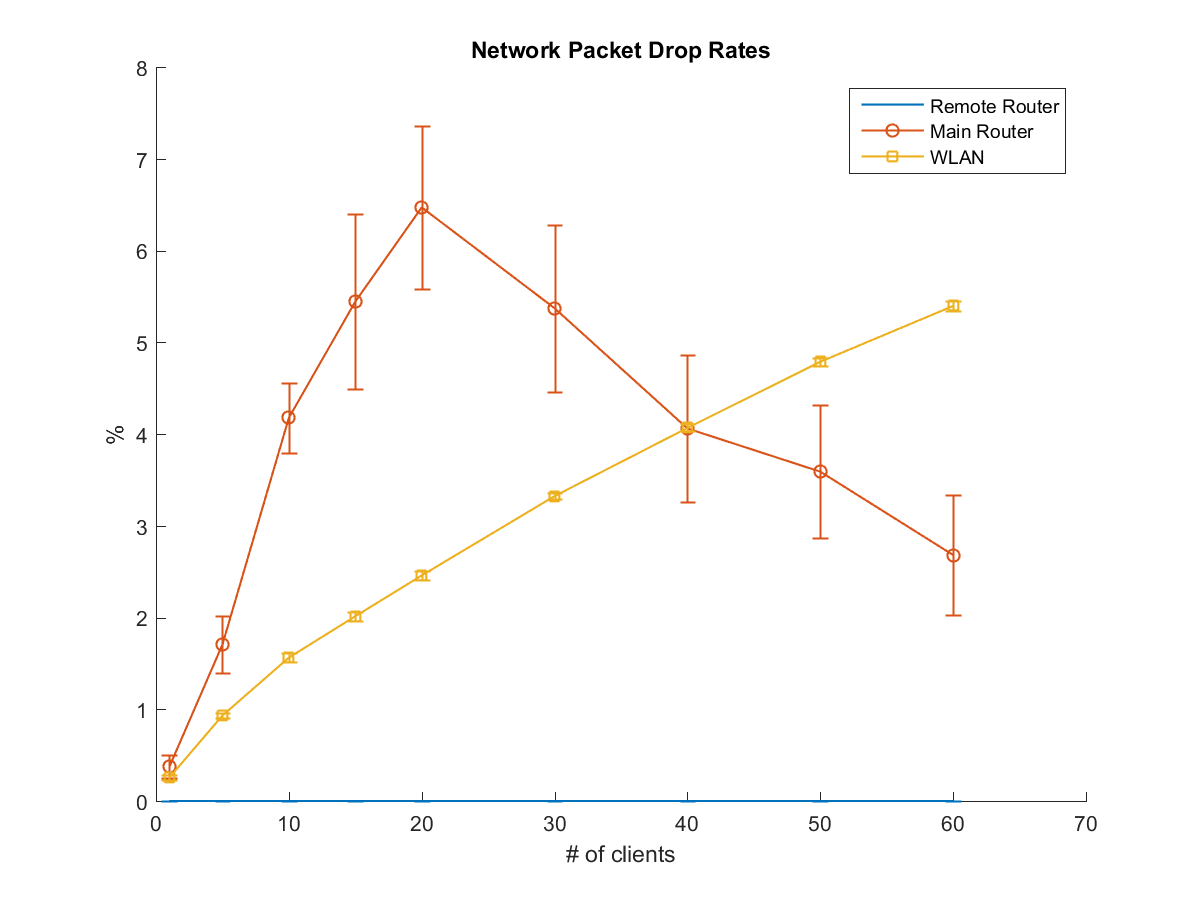
\includegraphics[width=\textwidth]{Figures/nocctv/Network_Packet_Drop_Rates.png}
  \caption{Packet drop rates at different points in the network} \label{fig:net_drop}
\end{figure}


The main bottleneck is the WLAN: as can be seen in fig. \ref{fig:net_throughput}, its throughput stagnates around 10 Mbit/s, staying below the 12 Mbit/s the radio link would theoretically be capable of transmitting. However, even the radio link itself is not fully occupied. One cause for this may be the drop rate of the Main Router that can be seen in fig. \ref{fig:net_drop} in combination with the increasing session durations shown in fig. \ref{fig:browser_sess_dur}: Until its peak at 20 Web Browsing Laptops, the Main Router is confronted with more traffic caused by HTTP responses and video conference data flowing from the professor to the remote site than it can handle. After 20 clients, the increased session duration has caused an overall smaller number of sessions to be active, resulting in fewer data to be transmitted by the Main Router through the radio link. While this relieves the Main Router's queue, it also decreases the overall throughput of the radio link.

\subsubsection{Maxmimum number of web browsing clients}
When the video conference is key,the maximum number of web browsing clients is reached when either the average packet loss exceeds the maximum of 5\% or the average delay exceeds the maximum of 100 ms.\\
Assuming client packet loss is linear starting at 10 clients, the video conference packet loss will exceed its maximum when $\geq$ 90 web browsing clients are present.
 Even at 60 clients, the delay measured at the Conference Laptop does not significantly exceed half of the permitted maximum delay of 100 ms, as can be seen in Fig. \ref{fig:ploss}.When assuming logarithmic growth, unacceptable packet loss rates will occur long before the maximum delay threshold is reached. \\

When taking the students' web browsing experience into account, however, the maximum number of clients is reached far quicker with the current setup. The acceptable response time of 10s is already reached with \textless 15 clients, as can be seen in fig. \ref{fig:browser_sess_dur}.% TODO: calculate exact number


\section{Recommended Changes To The Network}
%TODO: are there any things we'd recommend to be changed based on our simulations?
%TODO: wie kann man die video QoS verbessern, wie die browsing QoS?
%- mehr APs *auf unterschiedlichen channeln!* (da das WLAN medium sonst überlastet ist und zum bottleneck wird) -> ein AP pro 20 clients
%- gemeinsames updaten der WLAN und RadioLink bandwidth
%- begrenzung der wlan bandbreite pro client -> reduzierungdes FTP uploads, erhöhung des http throughputs
%- dringend: reduzierung der queue sizes
As shown in the previous section, the network at hand provides a satisfactory quality of service for video conference data with up to 90 students browsing the web in parallel. The web browsing experience, however, is sub-par as soon as $\geq$ 15 clients are active. This is due to the fact that the Remote Access Point cannot provide more than 10 Mbit/s of bandwidth and is therefore the main bottleneck.\\
Based on these findings, we recommend to install additional access points if more than 15 students are expected to be active in the network. With more access points installed, the bottleneck would shift to the radio link, which therefore would need to be upgraded as well.\\
Additionally, limiting the bandwidth available to each individual user may improve the overall surfing experience as it prevents users such as the FTP client from unfairly occupying the channel at any time.

%----------------------------------------------------------------------------------------
%   GLOSSARY ETC
%----------------------------------------------------------------------------------------
\newpage

\section{Distribution of tasks}

\begin{table}[H]
\begin{tabularx}{\textwidth}{ l l }
  \textbf{Simulation Implementation} & Lotte \\
  \textbf{Simulation Execution} & Alexander \\
  \textbf{Plotting} & Alexander \\
  \textbf{Introductory text} & Lotte \\
  \textbf{Simulation Plan text} & Alexander \\
  \textbf{Evaluation with CCTV} & Alexander \\
  \textbf{Evaluation without CCTV} & Lotte \\
\end{tabularx}
\end{table}

\listoffigures % Print the list of figures

\listoftables % Print the list of tables


%----------------------------------------------------------------------------------------
%   BIBLIOGRAPHY (if any)
%----------------------------------------------------------------------------------------

\renewcommand{\refname}{\spacedlowsmallcaps{References}} % For modifying the bibliography heading

\bibliographystyle{unsrt}

\bibliography{sample.bib} % The file containing the bibliography

%----------------------------------------------------------------------------------------

\end{document}